\documentclass{beamer}

\usepackage[english]{babel}
\usepackage{xcolor}
\usepackage{amsmath}
\usepackage{amssymb}
\usepackage{comment}

\usepackage{tikz}
\usepackage{pgfplots}
\usepackage{pgfplotstable}
\usetikzlibrary{plotmarks,arrows,shapes,backgrounds,positioning}

\usepackage{etoolbox} %% For If-statements
\usepackage{hyperref}

%\usefonttheme{serif}
%\usepackage{palatino}
\usetheme{Rochester}
\usecolortheme{beaver}
\beamertemplatenavigationsymbolsempty

\title{ 
    ~\\~\\ 
    {\huge AdaProp} 
    \\~\\
    {\large Adaptive Propositionalisation of Multi-Instance Data Towards Image Classification}
    \\~
}
\author{~\\~\\Siva~Manoharan\\~\\Supervisor:~Dr~Eibe~Frank}
\date{} %% no date

%% Customizing colours:
\newtoggle{normaltheme}
\newtoggle{darktheme}
\toggletrue{normaltheme}
\togglefalse{darktheme}

\definecolor{darkgreen}{RGB}{0, 170, 0}
\definecolor{darkorange}{RGB}{255, 147, 0}
\colorlet{primaryRed}{darkred!60!black}       %% For most Reds
\colorlet{secondaryRed}{darkred!80!black}     %% When Red is surrounded by grey
\colorlet{edgeGrey}{white!60!black}           %% For increasing apparent sharpness
\iftoggle{normaltheme}{
    \colorlet{bgWhite}{white!97!black}            %% Near white, for page backgrounds
    \colorlet{headerGrey}{white!90!black}         %% For Header backgrounds
    \colorlet{fillGrey}{white!72!black}           %% For filling areas, e.g. chart areas
    \colorlet{diagFillGrey}{white!92!black}       %% For filling diagram areas
}{
\iftoggle{darktheme}{
    \colorlet{bgWhite}{white!80!black}            %% Near white, for page backgrounds
    \colorlet{headerGrey}{white!75!black}         %% For Header backgrounds
    \colorlet{fillGrey}{white!58!black}           %% For filling areas, e.g. chart areas
    \colorlet{diagFillGrey}{white!75!black}       %% For filling diagram areas
}{ %% medium theme
    \colorlet{bgWhite}{white!90!black}            %% Near white, for page backgrounds
    \colorlet{headerGrey}{white!83!black}         %% For Header backgrounds
    \colorlet{fillGrey}{white!65!black}           %% For filling areas, e.g. chart areas
    \colorlet{diagFillGrey}{white!85!black}       %% For filling diagram areas
}
}
\setbeamercolor*{item}{fg=primaryRed}         %% Bullet points
\setbeamercolor{title}{fg=secondaryRed}       
\setbeamercolor{background canvas}{bg=bgWhite}
\setbeamercolor{headline}{bg=headerGrey}
\setbeamertemplate{headline}[text line]{%
  \begin{beamercolorbox}%
      [wd=\paperwidth,ht=2cm]{headline}%
  \end{beamercolorbox}%
}

%% A Macro for a image and a caption
%% args: image, caption
\newcommand{\CenteredImage}[1]{%
    \begin{center} 
        \includegraphics[scale=0.25]{img/#1}
    \end{center}
}

%% A Macro for a image and a caption in a column
%% args: image, caption
\newcommand{\ImageAndCaptionColumn}[2]{%
    \begin{column}{.5\textwidth}
        \begin{center} 
            \includegraphics[scale=0.25]{img/#1} \\~\\ 
            {\Large #2}
        \end{center} 
    \end{column}
}

%% A Macro for frame template: a bullet point above two images, each with caption
%% args: bullet-text, img-left, caption-left, img-right, caption-right
\newcommand{\TextAndTwoImageFrame}[5]{%
    %% Default spacing is too large for just one bullet point.
    %% Reduce it:
    \vspace{-0.5cm}    
    
    \begin{itemize}
        \item #1
    \end{itemize}
    
    \vspace{-0.5cm} %% again, reducing spacing
    
    %% Two columns of image+caption pairs:
    \begin{columns}[T]
        \ImageAndCaptionColumn{#2}{#3}
        \ImageAndCaptionColumn{#4}{#5}
    \end{columns}
}

%% A Macro for frame template: 3 bullet points
%% args: bullet1, bullet2, bullet3
\newcommand{\ThreeBulletFrame}[3]{%
    \begin{itemize}
        \item {#1} \\ ~
        \item {#2} \\ ~
        \item {#3}
    \end{itemize}
}

%% A Macro for a column and line graph for our datasets:
%% args: bg-label, bg-coords, fg-label, fg-coords ; where
%%    bg: background datapoints, fg: foreground datapoints.
\newcommand{\ColumnAndLineGraph}[4]{%
    \begin{axis}[
        %% Fixed size graph
        width=11cm, height=7cm, bar width=0.35cm,
%
        %% draw only left and bottom lines
        axis x line*=bottom, axis y line*=left, draw=edgeGrey,
%
        %% y-axis: 40-95, with major=10, minor=5
        ymin=40, ymax=95, minor y tick num=1,  ytick={50,60,70,80,90},
        axis y discontinuity=crunch, ylabel={Accuracy (\%)},
%
        %% x-axis: category axis
        symbolic x coords={atoms,bonds,chains,musk1,musk2,trx,tiger,fox,eleph,people,bikes,cars},
        xtick=data, x tick label style={rotate=90,anchor=east}, 
%
        %% Legend: at bottom right, place line first, then bar.
        reverse legend, legend pos=south east
    ]
 
        %% Background bar plot
        \addplot[ybar,fill=fillGrey, draw=edgeGrey, area legend] 
            coordinates {#2};
        \addlegendentry{#1}
        
        %% Foreground line plot
        \addplot+[ycomb,mark=-,draw=primaryRed,very thick,mark size=0.175cm, line legend] 
            coordinates {#4};
        \addlegendentry{#3}
    \end{axis}
}

%% A Macro for drawing a Bag Of Vectors inside a TikZpicture.
%% Args: 
%%    xEllipse, yEllipse, yTopDots, yFirstVec, 
%%    yMidDots, ySecondVec, yBottomDots, yLabel
\newcommand{\BagOfVectors}[8]{%
    \draw [dashed, fill=diagFillGrey, draw=edgeGrey, very thick] (#1,#2) ellipse (0.8cm and 1.9cm);
    \node at (#1,#3) { \Large $\vdots$ };
    \node at (#1,#4) {\large $\left\langle {X_i} \right\rangle$};
    \node at (#1,#5) { \Large $\vdots$ };
    \node at (#1,#6) {\large $\left\langle {X_j} \right\rangle$};
    \node at (#1,#7) { \Large $\vdots$ };        
    \node at (#1,#8) {\Large{}Bag of Instances~~~};
}

%% A Macro for horizontal, red, thick arrows.
%% Args: x-start, x-end, y-coord
\newcommand{\HorizArrow}[3]{%
    \path [->, primaryRed, ultra thick] (#1,#3) edge (#2,#3);
}

%% A Macro for vertical, red, thick arrows.
%% Args: x-coord, y-start, y-end, 
\newcommand{\VertArrow}[3]{%
    \path [->, primaryRed, ultra thick] (#1,#2) edge (#1,#3);
}

%% A Macro for horizontal, grey, thick arrows.
%% Args: x-start, x-end, y-coord
\newcommand{\HorizGreyArrow}[3]{%
    \path [->, edgeGrey, ultra thick] (#1,#3) edge (#2,#3);
}

%% A Macro for text nodes.
%% Args: xPos, yPos, text, text width, text depth
\newcommand{\TextNode}[5]{%
    \node[draw=edgeGrey, very thick, text width=#4, text depth=#5,
    	every text node part/.style={align=center}] 
    	at (#1, #2) {\Large #3};
}

%% A Macro for 90-degree rotated text nodes.
%% Args: xPos, yPos, text, text height, text depth
\newcommand{\RotatedTextNode}[5]{%
    \node[draw=edgeGrey, very thick, text height=#4, text depth=#5,
        rotate=90, text width=4.5cm,
        every text node part/.style={align=center}]
        at (#1, #2)
        {\Large #3};
}

%% A Macro for a filled rectangular box
%% Args: xPos, yPos, text height, text width
\newcommand{\FilledBox}[4]{%
    \node[draw=edgeGrey, fill=diagFillGrey, dashed, very thick, 
    	text height=#3, text width=#4] 
    	at (#1, #2) {};
}

%% A Macro for a dotted vertical line
%% Args: xPos, yStart, yEnd
\newcommand{\DottedVertLine}[3]{%
	\addplot[dashed, thick, sharp plot] coordinates {(#1, #2) (#1, #3)};
}

%% A Macro for a filled-in vertical line
%% Args: xPos, yStart, yEnd
\newcommand{\FullVertLine}[3]{%
	\addplot[primaryRed, very thick, sharp plot] coordinates {(#1, #2) (#1, #3)};
}

%% A Macro for a filled-in vertical line in grey
%% Args: xPos, yStart, yEnd
\newcommand{\GreyVertLine}[3]{%
	\addplot[edgeGrey, very thick, sharp plot] coordinates {(#1, #2) (#1, #3)};
}

%% A Macro for a dotted horizontal line
%% Args: xStart, xEnd, yPos
\newcommand{\DottedHoriLine}[3]{%
	\addplot[dashed, thick, sharp plot] coordinates {(#1, #3) (#2, #3)};
}

%% A Macro for a filled-in horizontal line
%% Args: xStart, xEnd, yPos
\newcommand{\FullHoriLine}[3]{%
	\addplot[primaryRed, very thick, sharp plot] coordinates {(#1, #3) (#2, #3)};
}

%% A Macro for a filled-in horizontal line in grey
%% Args: xStart, xEnd, yPos
\newcommand{\GreyHoriLine}[3]{%
	\addplot[edgeGrey, very thick, sharp plot] coordinates {(#1, #3) (#2, #3)};
}




\begin{document}

%% remove header bar for the titlepage
{
    \makeatletter
        \setbeamercolor{headline}{bg=bgWhite}
        \def\beamer@entrycode{\vspace*{-0.8\headheight}}
    \makeatother

    \begin{frame}
        \titlepage
    \end{frame}
}

\begin{frame}{Image Classification}

%% Application area: image classification ;
%% Given a object of interest, (cars), Given any image, 
%% We want to build software which can detect, whether or not, ...
%% This is binary image classification: what we want the software to output is 
%%	either positive - meaning ... (image) or negative - meaning ... (image)

    \TextAndTwoImageFrame{
    	Does the Image contain a specific object?
    }{cars1}{Car (Positive)}{none1}{No car (Negative)}
    
\end{frame}


\begin{frame}{Image Classification via Machine Learning}

%% We use a ML appr; we get a bunch of images, label them +ve/-ve;
%% Feed it into our ML algo : AdaProp ; which produces a model ; 
%% Which is basically some software is able to detect cars in the image with some degree of accuracy
%% So given any image, we can run it through the model, and it will output +ve/-ve
%% The model has learned how to detect cars

%% This is ML, so it works with any category of objects
%% In our training dataset, if we labelled bikes or persons as positive, 
%% What we get is a model which can detect if there is a person in the image

	\makebox[\linewidth]{\parbox{11.5cm}{%
        \begin{tikzpicture}%[every text node part/.style={align=center}]
        
		\def\yc{-2}; %% Vertical center        
		
		\def\trX{4.05}; %% X-coord of Training Dataset Node's rightmost border
		\def\mlX{5.00}; %% X-coord of ML Node's leftmost border
		\def\mrX{8.50}; %% X-coord of ML Node's rightmost border
		\def\olX{9.65}; %% X-coord of Model Node's leftmost border    

		\def\ocX{10.50}; %% X-center of Model Node
		\def\tbY{-1.05}; %% Y-coord of bottom of top-test-image
		\def\otY{-1.65}; %% Y-coord of Model Node's top border
		\def\obY{-2.30}; %% Y-coord of Model Node's bottom border
		\def\btY{-2.90}; %% Y-coord of top of bottom-test-image
		\def\olY{09.65}; %% X-coord of Model Node's leftmost border
        
        %% Diagram
        \FilledBox{2.025}{\yc}{4cm}{4.1cm}
        \only<1>{
        	\node [inner sep=0pt,below right] at (0,0) {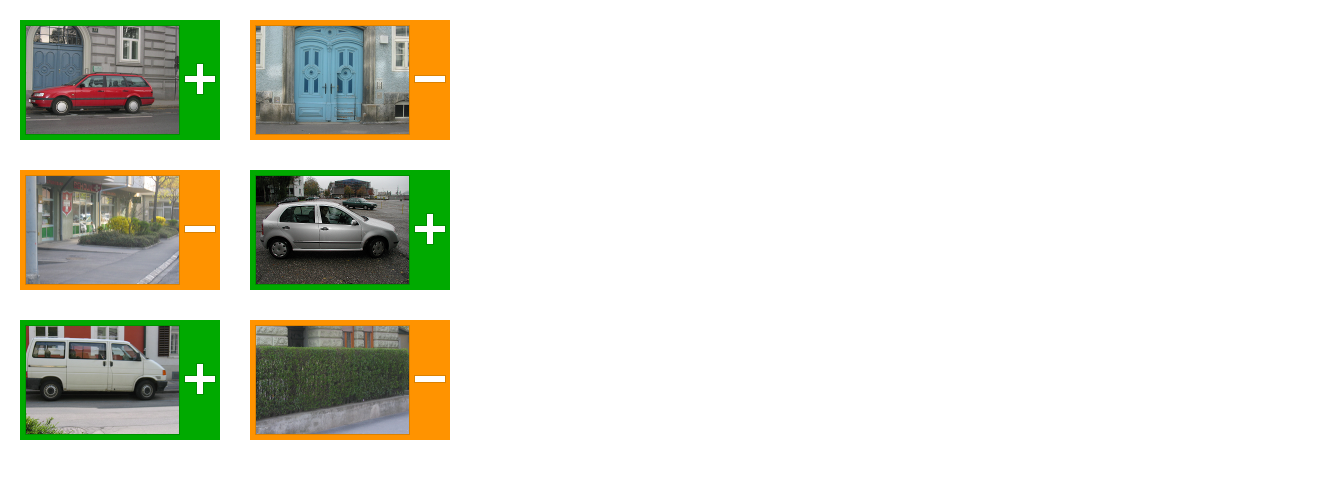
\includegraphics[scale=0.25]{img/ml1}};
        }
        \only<2>{
        	\node [inner sep=0pt,below right] at (0,0) {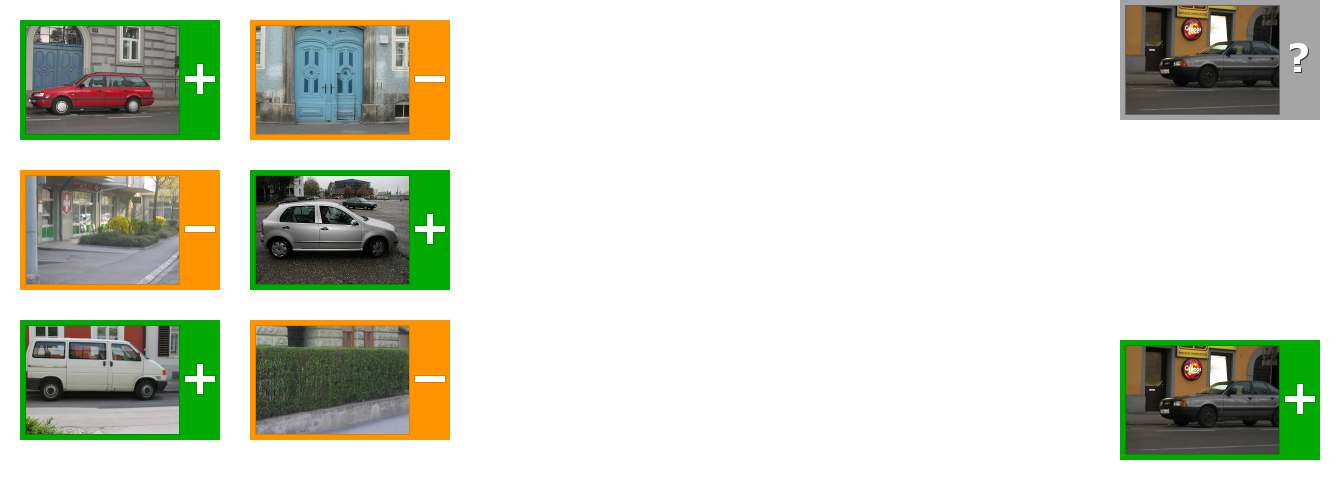
\includegraphics[scale=0.25]{img/ml2}};
        }
		\TextNode{6.75}{\yc}{Machine Learning Algorithm}{3.2cm}{1cm};
        \TextNode{10.495}{\yc}{Model}{1.425cm}{0cm};
                
		%% Arrows	
		\only<1>{
			\HorizArrow{\trX}{\mlX}{-1.5};
			\HorizArrow{\trX}{\mlX}{\yc};
			\HorizArrow{\trX}{\mlX}{-2.5};
			\HorizArrow{\mrX}{\olX}{\yc};
		}  
		\only<2>{
			\HorizGreyArrow{\trX}{\mlX}{-1.5};
			\HorizGreyArrow{\trX}{\mlX}{\yc};
			\HorizGreyArrow{\trX}{\mlX}{-2.5};
			\HorizGreyArrow{\mrX}{\olX}{\yc};
			\VertArrow{\ocX}{\tbY}{\otY};
			\VertArrow{\ocX}{\obY}{\btY};
		}  	            
                      
        %% Captions:
        \def\yCaption{-5};
        \node at (2.00, \yCaption) { \Large Training Dataset };
        \end{tikzpicture}
    }}

\end{frame}

\begin{frame}{Image Classification: Challenges}

%% Image classification is relatively easy for humans, but not for computers
%% The datasets we've been using have some challenging aspects.
%% For example, the relative size of the object of interest varies significantly between the images
%% (image) is 3k pix, 1%, while the other is 50%,
%% Also, the images can view the object from any orientation, front/back/side/ etc
%% Our process has to be able to ignore the scale and look for e.g. for cars of any scale and any orientation

    \TextAndTwoImageFrame{
    	Scale and Orientation
    }{size2}{150,000 pixels}{size1}{3,000 pixels}
    
\end{frame}


\begin{frame}{Image Classification: Challenges}

%% Another type of challenge is that the lighting conditions also vary significantly between images
%% On (image), taken at night, the lighting is obv. very low, while in the other (image), 
%% 	the reflection has washed out a lot of the details of the car
%% Our process has to somehow normalize between these conditions, it can't rely on pixel brightness alone
%%	for example.

\TextAndTwoImageFrame{
        Lighting Conditions
    }{light1}{Low light}{light2}{Overexposure}

\end{frame}

\begin{frame}{Image Classification: Challenges}

%% A more difficult type of challenge is partial occlusion, which occurs quite often in our dataset.
%% On some (images) the entire object is visible but some part is behind transparent objects
%%  like glass. So we can see the entire object, but part of it has color shifted
%% But in other cases, the object is blocked by opaque foreground objects, 
%%	so we actually cannot obtain the rest of the pixels of the object, only part.
%% Not only that, we cant obtain continous region of pix

    \TextAndTwoImageFrame{
        Partial Occlusion
    }{occl3}{Behind Glass}{occl1}{Obscured by Foreground}
    
\end{frame}

\begin{frame}{Multi-Instance Learning}

%% Those challenges mean that a global representation is not very effective
%% MIL allows us to say, if any subregion contains any part of the car, ...
    
    \vspace{-0.355cm}
    \begin{itemize}
        \item Natural fit for Image Classification %% (also Chemical, Text)
    \end{itemize}
    \vspace{0.215cm}
    
    \makebox[\linewidth]{\parbox{11.5cm}{%
        \begin{tikzpicture}%[every text node part/.style={align=center}]
        
        %% include the car picture
        \only<1>{
            \node [inner sep=0pt,below right] at (0,0) {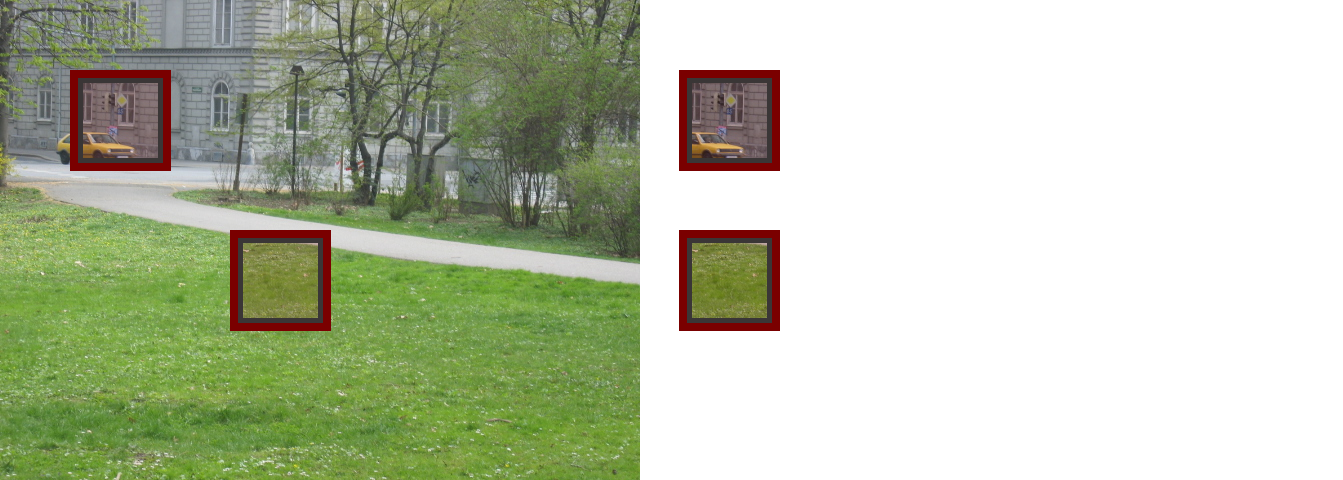
\includegraphics[scale=0.25]{img/cars4}};
        }
        \only<2>{
            \node [inner sep=0pt,below right] at (0,0) {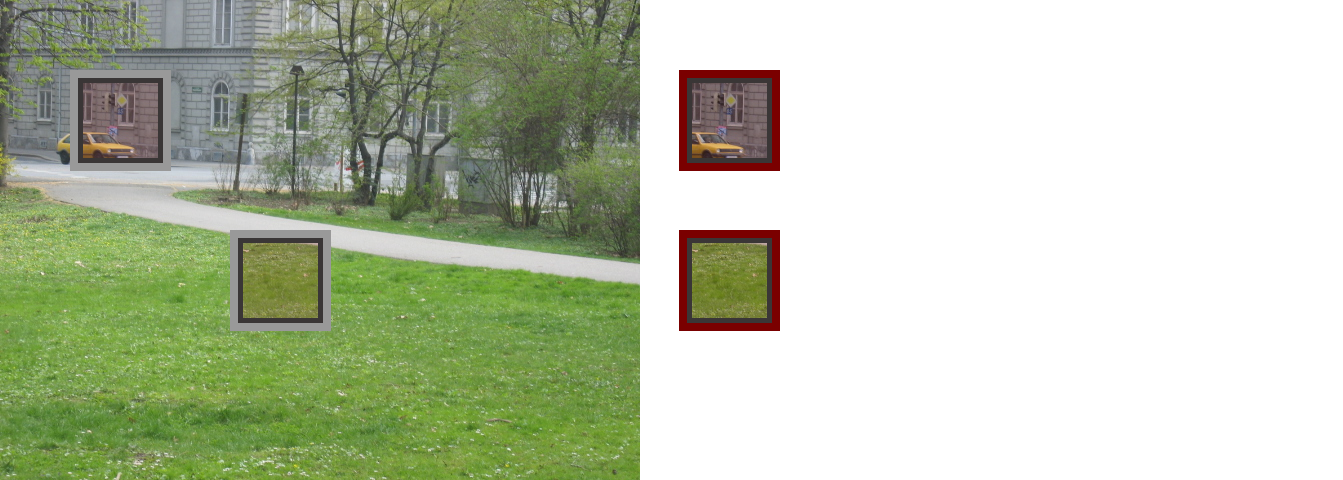
\includegraphics[scale=0.25]{img/cars5}};
        }
        
        %% Intermediate points
        \def\xZ{5.77};
        \def\xY{6.65};
        \def\xX{10.00};        
        
        %% Define some floats: 'A' near the car, 'B' away from the car
        \def\yA{-1.05};
        \def\yB{-2.40};
        
        %% Arrows from image to floats
        \only<1>{
            \HorizArrow{1.475}{\xZ}{\yA};
            \HorizArrow{2.845}{\xZ}{\yB};
        }
        \only<2>{
            \HorizGreyArrow{1.475}{\xZ}{\yA};
            \HorizGreyArrow{2.845}{\xZ}{\yB};
        }
      
        %% Captions:
        \def\yCaption{-5};
        \node at (3.00, \yCaption) { \Large Sub-regions };

        %% Draw the bag of vectors:
        \uncover<2>{
            \BagOfVectors{10.4}{-1.8}{-0.30}{-1.10}{-1.60}{-2.45}{-3.00}{\yCaption}
            \HorizArrow{\xY}{\xX}{\yA}; 
            \HorizArrow{\xY}{\xX}{\yB};    

            \node[%draw=edgeGrey, dashed, very thick,text height=1cm, text depth=1cm,
                text width=2.2cm, 
                every text node part/.style={align=center}] at (8.2, -1.7) 
                { \Large Feature Extraction };
        }
        \end{tikzpicture}
    }}

\end{frame}

\begin{frame}{Feature Extraction}
    \TextAndTwoImageFrame{
        Two well-known approaches
    }{feat1}{Local Binary Patterns}{feat2}{SURF Descriptor}
\end{frame}

\begin{frame}{Multi-Instance Learning}

%% Those challenges mean that a global representation is not very effective
%% MIL allows us to say, if any subregion contains any part of the car, ...
    
    \vspace{-0.355cm}
    \begin{itemize}
        \item Natural fit for Image Classification %% (also Chemical, Text)
    \end{itemize}
    \vspace{0.215cm}
    
    \makebox[\linewidth]{\parbox{11.5cm}{%
        \begin{tikzpicture}%[every text node part/.style={align=center}]
        
        %% include the car picture
        \node [inner sep=0pt,below right] at (0,0) {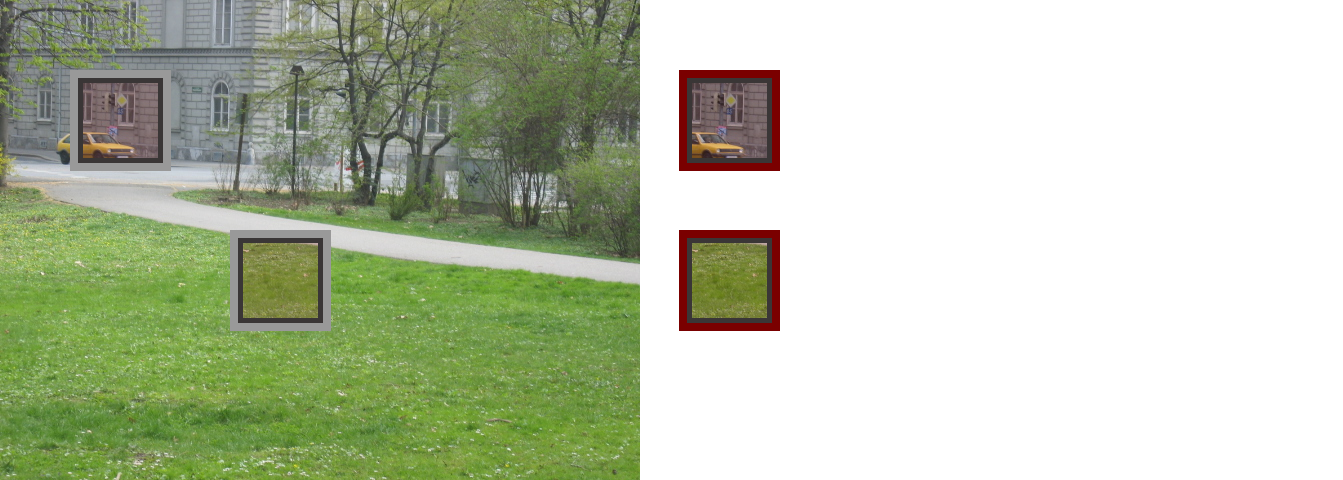
\includegraphics[scale=0.25]{img/cars5}};
                
        %% Intermediate points
        \def\xZ{5.77};
        \def\xY{6.65};
        \def\xX{10.00};        
        
        %% Define some floats: 'A' near the car, 'B' away from the car
        \def\yA{-1.05};
        \def\yB{-2.40};
        
        %% Arrows from image to floats
        \HorizGreyArrow{1.475}{\xZ}{\yA};
        \HorizGreyArrow{2.845}{\xZ}{\yB};
        
        %% Captions:
        \def\yCaption{-5};
        \node at (3.00, \yCaption) { \Large Sub-regions };

        %% Draw the bag of vectors:
        \BagOfVectors{10.4}{-1.8}{-0.30}{-1.10}{-1.60}{-2.45}{-3.00}{\yCaption}
        \HorizArrow{\xY}{\xX}{\yA}; 
        \HorizArrow{\xY}{\xX}{\yB};    

        \node[%draw=edgeGrey, dashed, very thick,text height=1cm, text depth=1cm,
        	text width=2.2cm, 
        	every text node part/.style={align=center}] at (8.2, -1.7) 
                { \Large Feature Extraction };
        
        \end{tikzpicture}
    }}

\end{frame}

\begin{frame}{Propositionalisation}

    \makebox[\linewidth]{\parbox{11.5cm}{%
        %\tikzstyle{background grid}=[draw, black!50,step=0.5cm]
        \begin{tikzpicture}%[show background grid]%[every text node part/.style={align=center}]
        
        %% Bag of vectors ellipse:
        \def\xEllipse{1.5};
        \def\yBase{-1.8};     
        \def\yCaption{-5};
        \BagOfVectors{\xEllipse}{\yBase}{-0.30}{-1.10}{-1.60}{-2.45}{-3.00}{\yCaption};
        
        %% Propositionalisation node:
        \def\xProp{4.5};
        \RotatedTextNode{\xProp}{\yBase}{Propositionalisation}{1cm}{0.7cm};
            
        %% Single vector circle:
        \def\xCirc{7.25};
        \draw [dashed, fill=diagFillGrey, draw=edgeGrey, very thick] (\xCirc,\yBase) circle (0.7cm);
        \node at (\xCirc,\yBase) { \large $\left\langle {Y} \right\rangle$ };
        \node at (\xCirc,\yCaption) { \Large Single Instance };
        
        %% Base Learner node:
        \RotatedTextNode{10}{\yBase}{Standard ML Algorithm}{0.85cm}{0.85cm};        
        
        %% Arrows:
        \def\yA{-1.095};
        \def\yB{-2.445};
        \def\xZ{1.90};
        \def\xY{3.45};
        \only<1>{
            \HorizArrow{\xZ}{\xY}{\yA};
            \HorizArrow{\xZ}{\xY}{\yB};
            \HorizArrow{5.50}{6.475}{\yBase};
            \HorizArrow{7.95}{8.95}{\yBase};
        }
        \only<2>{
            \HorizGreyArrow{\xZ}{\xY}{\yA};
            \HorizGreyArrow{\xZ}{\xY}{\yB};
            \HorizGreyArrow{5.50}{6.475}{\yBase};
            \HorizGreyArrow{7.95}{8.95}{\yBase};
        }
        
        
        %% Adaptive arrow
        \def\yAda{0};
        \only<2>{
            \frametitle{Adaptive Propositionalisation}       
        }
        \uncover<2>{
            \path [->, primaryRed, ultra thick, line width=0.1cm] (9,\yAda) edge (5.55,\yAda);
            \node[color=primaryRed] at (\xCirc,0.3) { \Large Adaptive };
        }
        
    \end{tikzpicture}
    }}
            
\end{frame}

\begin{comment}
\begin{frame}{Multi-Instance Learning}
    \ThreeBulletFrame
        {Natural for Image Classification}
        {Text Classification and Chemical datasets}
        {Key: Bags of Instances}
\end{frame}

\begin{frame}{Propositionalisation}
    \ThreeBulletFrame
        {Multi-instance $\to$ Single-instance}
        {Advantage: Existing algorithms}
        {Disadvantage: Lossy conversion}   
\end{frame}

\begin{frame}{AdaProp: Adaptive Propositionalisation}
    \ThreeBulletFrame
        {Use the base learner}
        {Tree of decisions / partitions}
        {Count by region}
\end{frame}
\end{comment}

\begin{frame}{AdaProp: Example Dataset}
%\begin{center}
\begin{tikzpicture}

	%% Image and Large marks
	\def\xImg{1.15};
	\def\ya{-0.840};
	\def\yb{-2.905};
	\def\yc{-4.965};
	\node [inner sep=0pt,below right] at (0,-0.025) {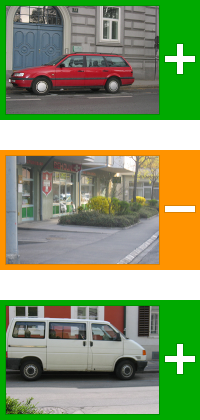
\includegraphics[scale=0.4]{img/eg1}};
	%\draw [mark=square*,mark size=5pt,mark options={color=darkgreen}] plot coordinates {(\xImg,\ya)};
	%\draw [mark=triangle*,mark size=5pt,mark options={color=darkorange}] plot coordinates {(\xImg,\yb)};
	%\draw [mark=*,mark size=5pt,mark options={color=darkgreen}] plot coordinates {(\xImg,\yc)};

\only<2>{
	%% Arrows
	\def\xA{2.8};
	\def\xB{4.35};
	\def\xC{6.0};
	\HorizArrow{\xA}{\xB}{\ya};
	\HorizArrow{\xA}{\xB}{\yb};
	\HorizArrow{\xA}{\xB}{\yc};

	%% Bags
	\def\ellX{1.5};
	\def\ellY{0.6};
	\draw [dashed, fill=diagFillGrey, draw=edgeGrey, very thick] (\xC,\ya) ellipse (\ellX cm and \ellY cm);
	\draw [dashed, fill=diagFillGrey, draw=edgeGrey, very thick] (\xC,\yb) ellipse (\ellX cm and \ellY cm);
	\draw [dashed, fill=diagFillGrey, draw=edgeGrey, very thick] (\xC,\yc) ellipse (\ellX cm and \ellY cm);
	
	%% Small marks
	\draw [mark=square*,mark size=3pt,mark options={color=darkgreen}] plot coordinates {(5.4,\ya)};
	\draw [mark=square*,mark size=3pt,mark options={color=darkgreen}] plot coordinates {(6.0,\ya)};
	\draw [mark=square*,mark size=3pt,mark options={color=darkgreen}] plot coordinates {(6.6,\ya)};
		
	\draw [mark=triangle*,mark size=3pt,mark options={color=darkorange}] plot coordinates {(5.1,\yb)};
	\draw [mark=triangle*,mark size=3pt,mark options={color=darkorange}] plot coordinates {(5.7,\yb)};
	\draw [mark=triangle*,mark size=3pt,mark options={color=darkorange}] plot coordinates {(6.3,\yb)};
	\draw [mark=triangle*,mark size=3pt,mark options={color=darkorange}] plot coordinates {(6.9,\yb)};
	
	\draw [mark=*,mark size=3pt,mark options={color=darkgreen}] plot coordinates {(5.4,\yc)};
	\draw [mark=*,mark size=3pt,mark options={color=darkgreen}] plot coordinates {(6.0,\yc)};
	\draw [mark=*,mark size=3pt,mark options={color=darkgreen}] plot coordinates {(6.6,\yc)};
	
	%% Captions
	\def\xD{9.5};
	\node[every text node part/.style={align=center}] at (\xD,\ya) {\Large 3 Instances};
	\node[every text node part/.style={align=center}] at (\xD,\yb) {\Large 4 Instances};
	\node[every text node part/.style={align=center}] at (\xD,\yc) {\Large 3 Instances};
}

\end{tikzpicture}
%\end{center}
\end{frame}

\begin{frame}{AdaProp: Example Dataset}
%\begin{center}
\begin{tikzpicture}

	\begin{axis}[xlabel={$a_1$}, ylabel={$a_2$}, xmin=0,xmax=1,ymin=0,ymax=1,
		 scatter/classes={p={mark=square*,darkgreen},q={darkgreen},n={mark=triangle*,darkorange}}]
		\addplot[scatter,only marks,scatter src=explicit symbolic] table[meta=label] {data/d1.dat};
		\only<2>{
			\DottedVertLine{0.4}{0}{1};
			\DottedVertLine{0.7}{0}{1};
			\DottedHoriLine{0}{1}{0.5};
		}
		\only<3->{ 
			\FullVertLine{0.4}{0}{1}; 
		}
		\only<4>{
			\DottedVertLine{0.15}{0}{1};
			\DottedHoriLine{0}{0.4}{0.2};
			\DottedHoriLine{0}{0.4}{0.5};
			\DottedVertLine{0.7}{0}{1};
			\DottedHoriLine{0.4}{1}{0.3};
			\DottedHoriLine{0.4}{1}{0.85};
		}
		\only<5->{ 
			\FullHoriLine{0}{0.4}{0.5};
			\FullHoriLine{0.4}{1}{0.85};
		}
	\end{axis}
	
	\def\xImg{8.75};
	\def\xLi{8};
	\node [inner sep=0pt,below right] at (\xLi,4.7) {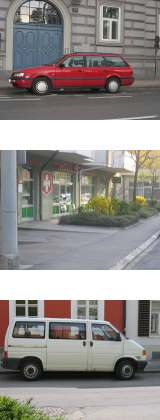
\includegraphics[scale=0.25]{img/eg2}};
	\draw [mark=square*,mark size=5pt,mark options={color=darkgreen}] plot coordinates {(\xImg,4.2)};
	\draw [mark=triangle*,mark size=5pt,mark options={color=darkorange}] plot coordinates {(\xImg,2.85)};
	\draw [mark=*,mark size=5pt,mark options={color=darkgreen}] plot coordinates {(\xImg,1.6)};
	
	
\end{tikzpicture}
%\end{center}
\end{frame}

%% Macros for the next slide-set.
\newcommand{\exampleImage}[1]{%
	\node [inner sep=0pt,below right] 
		at (7.5,5.5) 
		{\includegraphics[scale=0.167]{#1}};
}
\newcommand{\exampleVector}[4]{%
	\node[every text node part/.style={align=center}] 
		at (8.675,1.3) 
		{\Large $\left[\begin{array}{c} #1 \\ #2 \\ #3 \\ #4 \end{array}\right]$};
}
\newcommand{\exampleChart}[3]{%
	\begin{axis}[
			%yticklabels={,,}, xticklabels={,,}, 
			xlabel={$a_1$}, ylabel={$a_2$}, xmin=0,xmax=1,ymin=0,ymax=1,
			scatter/classes={p={mark=square*,#1},q={#3},n={mark=triangle*,#2}}
		]
		\addplot[scatter,only marks,scatter src=explicit symbolic] table[meta=label] {data/d1.dat};
		\GreyVertLine{0.4}{0}{1}; 
		\GreyHoriLine{0}{0.4}{0.5};
		\GreyHoriLine{0.4}{1}{0.85};		
	\end{axis}
}

\begin{frame}{AdaProp: Example Dataset}
%\begin{center}
\begin{tikzpicture}
	
	% The chart
	\only<1> { \exampleChart{darkgreen}{edgeGrey}{edgeGrey}; };
	\only<2> { \exampleChart{edgeGrey}{darkorange}{edgeGrey}; };
	\only<3> { \exampleChart{edgeGrey}{edgeGrey}{darkgreen}; };

	% Image
	\only<1> { \exampleImage{img/eg3}; };
	\only<2> { \exampleImage{img/eg4}; };
	\only<3> { \exampleImage{img/eg5}; };
	
	\def\xImg{8.65};
	\VertArrow{\xImg}{4.1}{2.7};
	
	% Propositionalised form (i.e. a vector)
	\only<1> { \exampleVector{1}{1}{1}{0}; };
	\only<2> { \exampleVector{0}{0}{1}{3}; };
	\only<3> { \exampleVector{1}{0}{1}{1}; };

\end{tikzpicture}
%\end{center}

\end{frame}


\begin{frame}[label=weka]{WEKA}
  \vspace{-0.5cm}
  \CenteredImage{weka3}
\end{frame}

\begin{frame}{AdaProp vs. Other MI algorithms}

    \begin{tikzpicture}
        \ColumnAndLineGraph{Others}{
            (atoms,83.90)  (bonds,87.96)  (chains,88.56)
            (musk1,90.68)  (musk2,85.89)  (trx,90.32)
            (tiger,84.30)  (fox,67.00)    (eleph,85.50)
            (people,82.60) (bikes,83.50)  (cars,77.22)
        }{AdaProp}{
            (atoms,87.52)  (bonds,89.44)  (chains,89.86)
            (musk1,85.76)  (musk2,82.26)  (trx,88.64)
            (tiger,84.20)  (fox,68.20)    (eleph,84.75)
            (people,81.88) (bikes,82.84)  (cars,77.08)
        }
    \end{tikzpicture}
    
\end{frame}

\begin{frame}{Summary}

  \begin{itemize}
  \item
      MI representation is \alert{natural} for Image Classification. \\ ~
  \item
      AdaProp propositionalises MI data using the \alert{base learner}. \\ ~
  \item
      \alert{Comparable performance} to other MI algorithms. % TODO need this?
  \end{itemize}
  
\end{frame}

\begin{frame}{Region Count Parameter Selection}
\begin{center}
\begin{tikzpicture}
	\begin{axis}[axis lines=left, yticklabels={,,}, xticklabels={,,},tick style={draw=none},
			xlabel={Number of Regions}, ylabel={Accuracy},
			xmin=0,xmax=1.1,ymin=0,ymax=1.1,
			legend pos= south east]
		\only<1-2>{
			\addplot[dashed,smooth,mark=none,black,very thick,domain=0.0:1] plot (\x,{1-exp(-6*\x)});
	    	\addlegendentry{Training~Set}
	    	\addlegendentry{Cross validated}
	    }
	    \only<2-> {
	    	\addplot[smooth,mark=none,primaryRed,very thick,domain=0.0:1] plot (\x,{0.8*sin(130*\x)});
	    }
	    \only<3>{
	    	\addplot[smooth,mark=none,black,very thick,domain=0.0:1] plot (\x,{0.95*sin(162*\x)});
	    	\addlegendentry{Dataset 1}
	    	\addlegendentry{Dataset 2}
	    }
	\end{axis}
\end{tikzpicture}
\end{center}
\end{frame}

\begin{comment}
\begin{frame}{Region count Parameter Selection}
    \ThreeBulletFrame
        {Too few regions $\to$ Underfitting}
        {Too many regions $\to$ Overfitting}
        {Optimal region count depends on dataset}
%% TODO: diagram for cross-validated parameter selection?
\end{frame}
\end{comment}

%\begin{comment}
\begin{frame}{Impact of Parameter Selection}

    \begin{tikzpicture}
        \ColumnAndLineGraph{Without}{
            (atoms,77.14)  (bonds,84.40)  (chains,85.81)
            (musk1,73.39)  (musk2,73.30)  (trx,85.36)
            (tiger,75.70)  (fox,65.95)    (eleph,73.30)
            (people,75.6)  (bikes,75.35)  (cars,68.54)
        }{With ParamSel}{
            (atoms,84.49)  (bonds,87.48)  (chains,86.60)
            (musk1,76.28)  (musk2,74.48)  (trx,86.61)
            (tiger,79.60)  (fox,65.95)    (eleph,75.90)
            (people,76.27) (bikes,77.24)  (cars,68.76)
        }
    \end{tikzpicture} 

\end{frame}
%\end{comment}

\begin{frame}{WEKA}
  \vspace{-0.5cm}
  \CenteredImage{weka3}
\end{frame}

\begin{frame}{Summary}

  \begin{itemize}
  \item
      MI representation is \alert{natural} for Image Classification. \\ ~
  \item
      AdaProp propositionalises MI data using the \alert{base learner}. \\ ~
  \item
      \alert{Comparable performance} to other MI algorithms. % TODO need this?
  \end{itemize}
  
\end{frame}

\end{document}


